\documentclass{standalone}
\usepackage{tikz}
\usetikzlibrary{patterns}
\usetikzlibrary{positioning}
\usetikzlibrary{patterns, positioning}
\usetikzlibrary{shapes.misc}
\usepackage[outline]{contour}
\contourlength{1.5pt} 
\usetikzlibrary{calc}
        \usepackage{relsize}
        \tikzset{fontscale/.style = {font=\relsize{#1}}}

\begin{document}
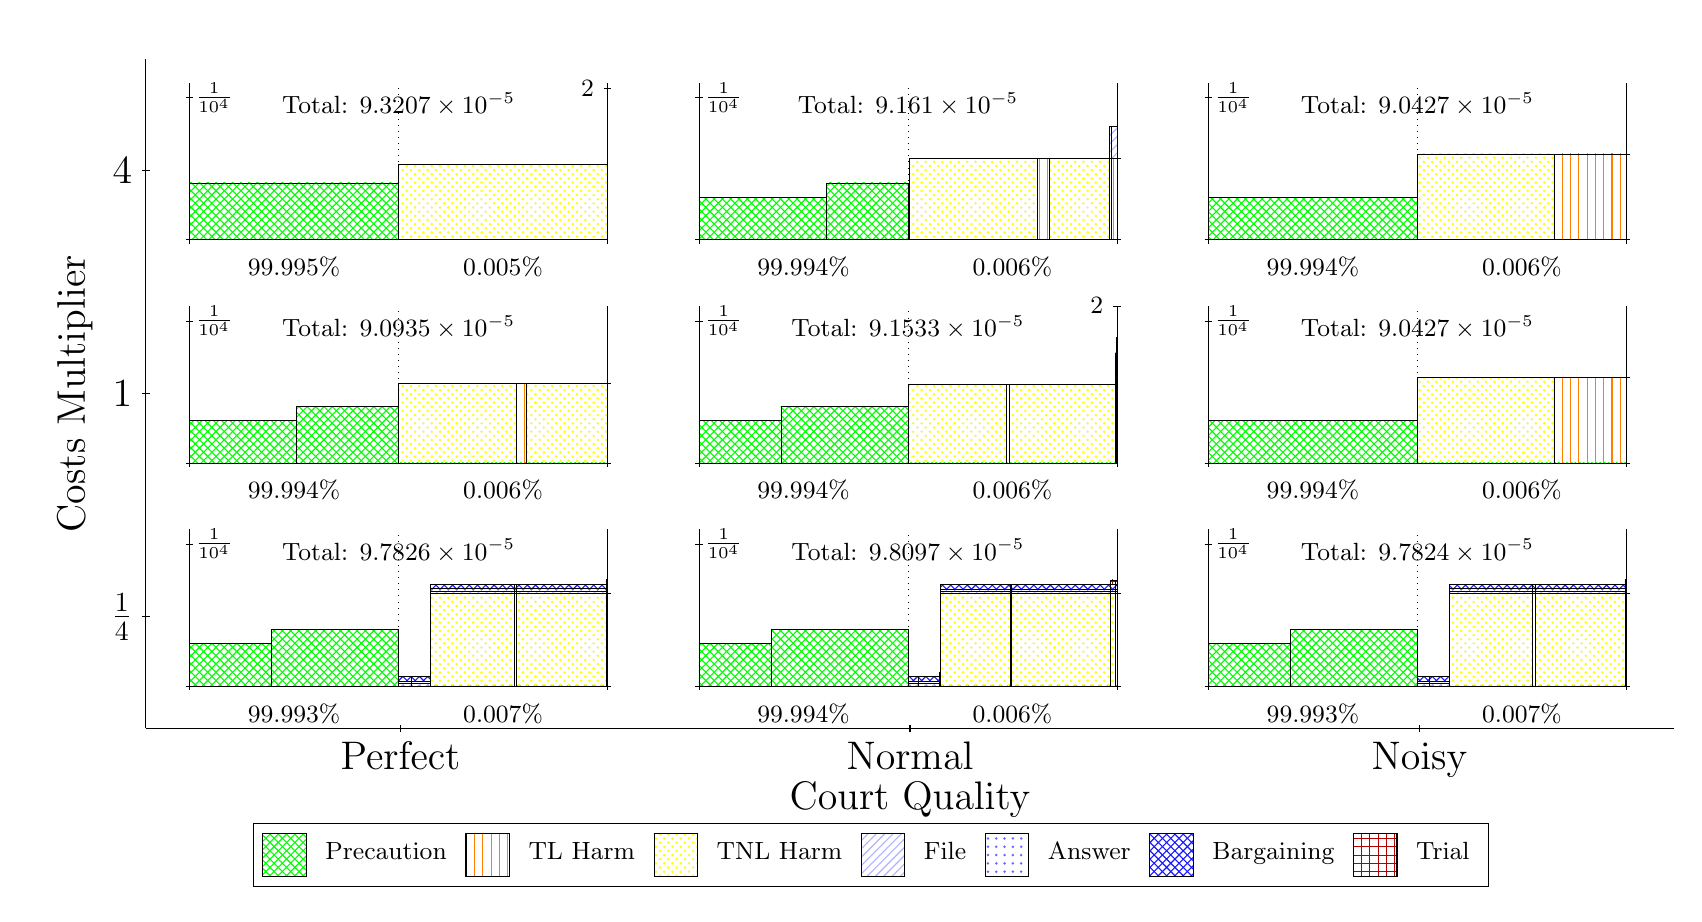
\begin{tikzpicture}
\clip(-0.5,-1.1) rectangle +(20.91,11);
\draw[black] (1,1) -- (1,9.5);
\node[rotate=90, fontscale=2, anchor=center] at (0.1, 5.25) {Costs Multiplier};
\draw[black] (0.95,2.4167) -- (1.05,2.4167);
\node[fontscale=2, anchor=east] at (0.95, 2.4167) {$\frac{1}{4}$};
\draw[black] (0.95,5.25) -- (1.05,5.25);
\node[fontscale=2, anchor=east] at (0.95, 5.25) {1};
\draw[black] (0.95,8.0833) -- (1.05,8.0833);
\node[fontscale=2, anchor=east] at (0.95, 8.0833) {4};

\draw[black] (1,1) -- (20.41,1);
\node[fontscale=2, anchor=center] at (10.705, 0.1) {Court Quality};
\draw[black] (4.235,0.95) -- (4.235,1.05);
\node[fontscale=2, anchor=north] at (4.235, 0.95) {Perfect};
\draw[black] (10.705,0.95) -- (10.705,1.05);
\node[fontscale=2, anchor=north] at (10.705, 0.95) {Normal};
\draw[black] (17.175,0.95) -- (17.175,1.05);
\node[fontscale=2, anchor=north] at (17.175, 0.95) {Noisy};


\draw[pattern=crosshatch, pattern color=green,draw=black,very thin] (1.5556,1.54) rectangle (2.5958,2.0809);
\draw[pattern=crosshatch, pattern color=green,draw=black,very thin] (2.5958,1.54) rectangle (4.21,2.2612);
\draw[pattern=crosshatch, pattern color=green,draw=black,very thin] (4.21,1.54) rectangle (4.3657,1.54);
\draw[pattern=north east lines, pattern color=blue!30,draw=black,very thin] (4.21,1.54) rectangle (4.3657,1.5694);
\draw[pattern=dots,  pattern color=blue!60,draw=black,very thin] (4.21,1.5694) rectangle (4.3657,1.5988);
\draw[pattern=crosshatch,      pattern color=blue!90,draw=black,very thin] (4.21,1.5988) rectangle (4.3657,1.6576);
\draw[pattern=crosshatch, pattern color=green,draw=black,very thin] (4.3657,1.54) rectangle (4.6133,1.54);
\draw[pattern=north east lines, pattern color=blue!30,draw=black,very thin] (4.3657,1.54) rectangle (4.6133,1.5694);
\draw[pattern=dots,  pattern color=blue!60,draw=black,very thin] (4.3657,1.5694) rectangle (4.6133,1.5988);
\draw[pattern=crosshatch,      pattern color=blue!90,draw=black,very thin] (4.3657,1.5988) rectangle (4.6133,1.6576);
\draw[pattern=crosshatch, pattern color=green,draw=black,very thin] (4.6133,1.54) rectangle (4.6172,1.54);
\draw[pattern=north east lines, pattern color=blue!30,draw=black,very thin] (4.6133,1.54) rectangle (4.6172,1.5694);
\draw[pattern=dots,  pattern color=blue!60,draw=black,very thin] (4.6133,1.5694) rectangle (4.6172,1.5988);
\draw[pattern=crosshatch,      pattern color=blue!90,draw=black,very thin] (4.6133,1.5988) rectangle (4.6172,1.6576);
\draw[pattern=grid,            pattern color=red!70!black,draw=black,very thin] (4.6133,1.6576) rectangle (4.6172,1.7164);
\draw[pattern=crosshatch, pattern color=green,draw=black,very thin] (4.6172,1.54) rectangle (5.6753,1.54);
\draw[pattern=crosshatch dots, pattern color=yellow,draw=black,very thin] (4.6172,1.54) rectangle (5.6753,2.7156);
\draw[pattern=north east lines, pattern color=blue!30,draw=black,very thin] (4.6172,2.7156) rectangle (5.6753,2.745);
\draw[pattern=dots,  pattern color=blue!60,draw=black,very thin] (4.6172,2.745) rectangle (5.6753,2.7744);
\draw[pattern=crosshatch,      pattern color=blue!90,draw=black,very thin] (4.6172,2.7744) rectangle (5.6753,2.8332);
\draw[pattern=crosshatch, pattern color=green,draw=black,very thin] (5.6753,1.54) rectangle (5.7003,1.54);
\draw[pattern=vertical lines, pattern color=orange,draw=black,very thin] (5.6753,1.54) rectangle (5.7003,2.7156);
\draw[pattern=north east lines, pattern color=blue!30,draw=black,very thin] (5.6753,2.7156) rectangle (5.7003,2.745);
\draw[pattern=dots,  pattern color=blue!60,draw=black,very thin] (5.6753,2.745) rectangle (5.7003,2.7744);
\draw[pattern=crosshatch,      pattern color=blue!90,draw=black,very thin] (5.6753,2.7744) rectangle (5.7003,2.8332);
\draw[pattern=crosshatch, pattern color=green,draw=black,very thin] (5.7003,1.54) rectangle (6.8428,1.54);
\draw[pattern=crosshatch dots, pattern color=yellow,draw=black,very thin] (5.7003,1.54) rectangle (6.8428,2.7156);
\draw[pattern=north east lines, pattern color=blue!30,draw=black,very thin] (5.7003,2.7156) rectangle (6.8428,2.745);
\draw[pattern=dots,  pattern color=blue!60,draw=black,very thin] (5.7003,2.745) rectangle (6.8428,2.7744);
\draw[pattern=crosshatch,      pattern color=blue!90,draw=black,very thin] (5.7003,2.7744) rectangle (6.8428,2.8332);
\draw[pattern=crosshatch, pattern color=green,draw=black,very thin] (6.8428,1.54) rectangle (6.8544,1.54);
\draw[pattern=crosshatch dots, pattern color=yellow,draw=black,very thin] (6.8428,1.54) rectangle (6.8544,2.7156);
\draw[pattern=north east lines, pattern color=blue!30,draw=black,very thin] (6.8428,2.7156) rectangle (6.8544,2.745);
\draw[pattern=dots,  pattern color=blue!60,draw=black,very thin] (6.8428,2.745) rectangle (6.8544,2.7744);
\draw[pattern=crosshatch,      pattern color=blue!90,draw=black,very thin] (6.8428,2.7744) rectangle (6.8544,2.8332);
\draw[pattern=grid,            pattern color=red!70!black,draw=black,very thin] (6.8428,2.8332) rectangle (6.8544,2.892);
\draw[pattern=crosshatch, pattern color=green,draw=black,very thin] (6.8544,1.54) rectangle (6.8644,1.54);
\draw[pattern=vertical lines, pattern color=orange,draw=black,very thin] (6.8544,1.54) rectangle (6.8644,2.7156);
\draw[pattern=north east lines, pattern color=blue!30,draw=black,very thin] (6.8544,2.7156) rectangle (6.8644,2.745);
\draw[pattern=dots,  pattern color=blue!60,draw=black,very thin] (6.8544,2.745) rectangle (6.8644,2.7744);
\draw[pattern=crosshatch,      pattern color=blue!90,draw=black,very thin] (6.8544,2.7744) rectangle (6.8644,2.8332);
\draw[pattern=grid,            pattern color=red!70!black,draw=black,very thin] (6.8544,2.8332) rectangle (6.8644,2.892);
\node[font=\small,text=black,anchor=north] at (4.21, 3.5333) {Total: $9.7826\times 10^{-5}$};
\draw[black,very thin] (1.5556,1.54) -- (1.5556,3.5333);
\draw[black,very thin] (1.5056,1.54) -- (1.6056,1.54);
\node[font=\small,text=black, anchor=west] at (1.5056, 1.54) {};
\draw[black,very thin] (1.5056,3.3431) -- (1.6056,3.3431);
\node[font=\small,text=black, anchor=west] at (1.5056, 3.3431) {$\frac{1}{10^{4}}$};

\draw[black,dotted,very thin] (4.21,1.5998) -- (4.21,3.4735);
\draw[black,very thin] (6.8644,1.54) -- (6.8644,3.5333);
\draw[black,very thin] (6.8144,1.54) -- (6.9144,1.54);
\node[font=\small,text=black, anchor=east] at (6.8144, 1.54) {\contour{white}{}};
\draw[black,very thin] (6.8144,2.7156) -- (6.9144,2.7156);
\node[font=\small,text=black, anchor=east] at (6.8144, 2.7156) {\contour{white}{}};

\draw[black,very thin] (1.5556,1.54) -- (6.8644,1.54);
\draw[black,very thin] (1.5556,1.49) -- (1.5556,1.59);
\node[font=\small,text=black, anchor=north] at (1.5556, 1.49) {};
\draw[black,very thin] (6.8644,1.49) -- (6.8644,1.59);
\node[font=\small,text=black, anchor=north] at (6.8644, 1.49) {};

\node[font=\small,text=black,anchor=south] at (2.8828, 0.94) {99.993\%};
\node[font=\small,text=black,anchor=south] at (5.5372, 0.94) {0.007\%};

\draw[pattern=crosshatch, pattern color=green,draw=black,very thin] (8.0256,1.54) rectangle (8.9441,2.0809);
\draw[pattern=crosshatch, pattern color=green,draw=black,very thin] (8.9441,1.54) rectangle (10.68,2.2612);
\draw[pattern=crosshatch, pattern color=green,draw=black,very thin] (10.68,1.54) rectangle (10.807,1.54);
\draw[pattern=north east lines, pattern color=blue!30,draw=black,very thin] (10.68,1.54) rectangle (10.807,1.5693);
\draw[pattern=dots,  pattern color=blue!60,draw=black,very thin] (10.68,1.5693) rectangle (10.807,1.5986);
\draw[pattern=crosshatch,      pattern color=blue!90,draw=black,very thin] (10.68,1.5986) rectangle (10.807,1.6571);
\draw[pattern=crosshatch, pattern color=green,draw=black,very thin] (10.807,1.54) rectangle (11.075,1.54);
\draw[pattern=north east lines, pattern color=blue!30,draw=black,very thin] (10.807,1.54) rectangle (11.075,1.5693);
\draw[pattern=dots,  pattern color=blue!60,draw=black,very thin] (10.807,1.5693) rectangle (11.075,1.5986);
\draw[pattern=crosshatch,      pattern color=blue!90,draw=black,very thin] (10.807,1.5986) rectangle (11.075,1.6572);
\draw[pattern=crosshatch, pattern color=green,draw=black,very thin] (11.075,1.54) rectangle (11.089,1.54);
\draw[pattern=north east lines, pattern color=blue!30,draw=black,very thin] (11.075,1.54) rectangle (11.089,1.5693);
\draw[pattern=dots,  pattern color=blue!60,draw=black,very thin] (11.075,1.5693) rectangle (11.089,1.5986);
\draw[pattern=crosshatch,      pattern color=blue!90,draw=black,very thin] (11.075,1.5986) rectangle (11.089,1.6571);
\draw[pattern=grid,            pattern color=red!70!black,draw=black,very thin] (11.075,1.6571) rectangle (11.089,1.7157);
\draw[pattern=crosshatch, pattern color=green,draw=black,very thin] (11.089,1.54) rectangle (11.979,1.54);
\draw[pattern=crosshatch dots, pattern color=yellow,draw=black,very thin] (11.089,1.54) rectangle (11.979,2.7111);
\draw[pattern=north east lines, pattern color=blue!30,draw=black,very thin] (11.089,2.7111) rectangle (11.979,2.7404);
\draw[pattern=dots,  pattern color=blue!60,draw=black,very thin] (11.089,2.7404) rectangle (11.979,2.7696);
\draw[pattern=crosshatch,      pattern color=blue!90,draw=black,very thin] (11.089,2.7696) rectangle (11.979,2.8282);
\draw[pattern=crosshatch, pattern color=green,draw=black,very thin] (11.979,1.54) rectangle (11.987,1.54);
\draw[pattern=vertical lines, pattern color=orange,draw=black,very thin] (11.979,1.54) rectangle (11.987,2.7111);
\draw[pattern=north east lines, pattern color=blue!30,draw=black,very thin] (11.979,2.7111) rectangle (11.987,2.7404);
\draw[pattern=dots,  pattern color=blue!60,draw=black,very thin] (11.979,2.7404) rectangle (11.987,2.7696);
\draw[pattern=crosshatch,      pattern color=blue!90,draw=black,very thin] (11.979,2.7696) rectangle (11.987,2.8282);
\draw[pattern=crosshatch, pattern color=green,draw=black,very thin] (11.987,1.54) rectangle (13.25,1.54);
\draw[pattern=crosshatch dots, pattern color=yellow,draw=black,very thin] (11.987,1.54) rectangle (13.25,2.7111);
\draw[pattern=north east lines, pattern color=blue!30,draw=black,very thin] (11.987,2.7111) rectangle (13.25,2.7404);
\draw[pattern=dots,  pattern color=blue!60,draw=black,very thin] (11.987,2.7404) rectangle (13.25,2.7697);
\draw[pattern=crosshatch,      pattern color=blue!90,draw=black,very thin] (11.987,2.7697) rectangle (13.25,2.8282);
\draw[pattern=crosshatch, pattern color=green,draw=black,very thin] (13.25,1.54) rectangle (13.313,1.54);
\draw[pattern=crosshatch dots, pattern color=yellow,draw=black,very thin] (13.25,1.54) rectangle (13.313,2.7111);
\draw[pattern=north east lines, pattern color=blue!30,draw=black,very thin] (13.25,2.7111) rectangle (13.313,2.7404);
\draw[pattern=dots,  pattern color=blue!60,draw=black,very thin] (13.25,2.7404) rectangle (13.313,2.7696);
\draw[pattern=crosshatch,      pattern color=blue!90,draw=black,very thin] (13.25,2.7696) rectangle (13.313,2.8282);
\draw[pattern=grid,            pattern color=red!70!black,draw=black,very thin] (13.25,2.8282) rectangle (13.313,2.8868);
\draw[pattern=crosshatch, pattern color=green,draw=black,very thin] (13.313,1.54) rectangle (13.334,1.54);
\draw[pattern=vertical lines, pattern color=orange,draw=black,very thin] (13.313,1.54) rectangle (13.334,2.7111);
\draw[pattern=north east lines, pattern color=blue!30,draw=black,very thin] (13.313,2.7111) rectangle (13.334,2.7404);
\draw[pattern=dots,  pattern color=blue!60,draw=black,very thin] (13.313,2.7404) rectangle (13.334,2.7696);
\draw[pattern=crosshatch,      pattern color=blue!90,draw=black,very thin] (13.313,2.7696) rectangle (13.334,2.8282);
\draw[pattern=grid,            pattern color=red!70!black,draw=black,very thin] (13.313,2.8282) rectangle (13.334,2.8868);
\node[font=\small,text=black,anchor=north] at (10.68, 3.5333) {Total: $9.8097\times 10^{-5}$};
\draw[black,very thin] (8.0256,1.54) -- (8.0256,3.5333);
\draw[black,very thin] (7.9756,1.54) -- (8.0756,1.54);
\node[font=\small,text=black, anchor=west] at (7.9756, 1.54) {};
\draw[black,very thin] (7.9756,3.3431) -- (8.0756,3.3431);
\node[font=\small,text=black, anchor=west] at (7.9756, 3.3431) {$\frac{1}{10^{4}}$};

\draw[black,dotted,very thin] (10.68,1.5998) -- (10.68,3.4735);
\draw[black,very thin] (13.334,1.54) -- (13.334,3.5333);
\draw[black,very thin] (13.284,1.54) -- (13.384,1.54);
\node[font=\small,text=black, anchor=east] at (13.284, 1.54) {\contour{white}{}};
\draw[black,very thin] (13.284,2.7111) -- (13.384,2.7111);
\node[font=\small,text=black, anchor=east] at (13.284, 2.7111) {\contour{white}{}};

\draw[black,very thin] (8.0256,1.54) -- (13.334,1.54);
\draw[black,very thin] (8.0256,1.49) -- (8.0256,1.59);
\node[font=\small,text=black, anchor=north] at (8.0256, 1.49) {};
\draw[black,very thin] (13.334,1.49) -- (13.334,1.59);
\node[font=\small,text=black, anchor=north] at (13.334, 1.49) {};

\node[font=\small,text=black,anchor=south] at (9.3528, 0.94) {99.994\%};
\node[font=\small,text=black,anchor=south] at (12.007, 0.94) {0.006\%};

\draw[pattern=crosshatch, pattern color=green,draw=black,very thin] (14.496,1.54) rectangle (15.536,2.0809);
\draw[pattern=crosshatch, pattern color=green,draw=black,very thin] (15.536,1.54) rectangle (17.15,2.2612);
\draw[pattern=crosshatch, pattern color=green,draw=black,very thin] (17.15,1.54) rectangle (17.306,1.54);
\draw[pattern=north east lines, pattern color=blue!30,draw=black,very thin] (17.15,1.54) rectangle (17.306,1.5694);
\draw[pattern=dots,  pattern color=blue!60,draw=black,very thin] (17.15,1.5694) rectangle (17.306,1.5988);
\draw[pattern=crosshatch,      pattern color=blue!90,draw=black,very thin] (17.15,1.5988) rectangle (17.306,1.6576);
\draw[pattern=crosshatch, pattern color=green,draw=black,very thin] (17.306,1.54) rectangle (17.553,1.54);
\draw[pattern=north east lines, pattern color=blue!30,draw=black,very thin] (17.306,1.54) rectangle (17.553,1.5694);
\draw[pattern=dots,  pattern color=blue!60,draw=black,very thin] (17.306,1.5694) rectangle (17.553,1.5988);
\draw[pattern=crosshatch,      pattern color=blue!90,draw=black,very thin] (17.306,1.5988) rectangle (17.553,1.6576);
\draw[pattern=crosshatch, pattern color=green,draw=black,very thin] (17.553,1.54) rectangle (17.557,1.54);
\draw[pattern=north east lines, pattern color=blue!30,draw=black,very thin] (17.553,1.54) rectangle (17.557,1.5694);
\draw[pattern=dots,  pattern color=blue!60,draw=black,very thin] (17.553,1.5694) rectangle (17.557,1.5988);
\draw[pattern=crosshatch,      pattern color=blue!90,draw=black,very thin] (17.553,1.5988) rectangle (17.557,1.6576);
\draw[pattern=grid,            pattern color=red!70!black,draw=black,very thin] (17.553,1.6576) rectangle (17.557,1.7164);
\draw[pattern=crosshatch, pattern color=green,draw=black,very thin] (17.557,1.54) rectangle (18.612,1.54);
\draw[pattern=crosshatch dots, pattern color=yellow,draw=black,very thin] (17.557,1.54) rectangle (18.612,2.7156);
\draw[pattern=north east lines, pattern color=blue!30,draw=black,very thin] (17.557,2.7156) rectangle (18.612,2.745);
\draw[pattern=dots,  pattern color=blue!60,draw=black,very thin] (17.557,2.745) rectangle (18.612,2.7744);
\draw[pattern=crosshatch,      pattern color=blue!90,draw=black,very thin] (17.557,2.7744) rectangle (18.612,2.8332);
\draw[pattern=crosshatch, pattern color=green,draw=black,very thin] (18.612,1.54) rectangle (18.64,1.54);
\draw[pattern=vertical lines, pattern color=orange,draw=black,very thin] (18.612,1.54) rectangle (18.64,2.7156);
\draw[pattern=north east lines, pattern color=blue!30,draw=black,very thin] (18.612,2.7156) rectangle (18.64,2.745);
\draw[pattern=dots,  pattern color=blue!60,draw=black,very thin] (18.612,2.745) rectangle (18.64,2.7744);
\draw[pattern=crosshatch,      pattern color=blue!90,draw=black,very thin] (18.612,2.7744) rectangle (18.64,2.8332);
\draw[pattern=crosshatch, pattern color=green,draw=black,very thin] (18.64,1.54) rectangle (19.783,1.54);
\draw[pattern=crosshatch dots, pattern color=yellow,draw=black,very thin] (18.64,1.54) rectangle (19.783,2.7156);
\draw[pattern=north east lines, pattern color=blue!30,draw=black,very thin] (18.64,2.7156) rectangle (19.783,2.745);
\draw[pattern=dots,  pattern color=blue!60,draw=black,very thin] (18.64,2.745) rectangle (19.783,2.7744);
\draw[pattern=crosshatch,      pattern color=blue!90,draw=black,very thin] (18.64,2.7744) rectangle (19.783,2.8332);
\draw[pattern=crosshatch, pattern color=green,draw=black,very thin] (19.783,1.54) rectangle (19.793,1.54);
\draw[pattern=crosshatch dots, pattern color=yellow,draw=black,very thin] (19.783,1.54) rectangle (19.793,2.7156);
\draw[pattern=north east lines, pattern color=blue!30,draw=black,very thin] (19.783,2.7156) rectangle (19.793,2.745);
\draw[pattern=dots,  pattern color=blue!60,draw=black,very thin] (19.783,2.745) rectangle (19.793,2.7744);
\draw[pattern=crosshatch,      pattern color=blue!90,draw=black,very thin] (19.783,2.7744) rectangle (19.793,2.8332);
\draw[pattern=grid,            pattern color=red!70!black,draw=black,very thin] (19.783,2.8332) rectangle (19.793,2.8919);
\draw[pattern=crosshatch, pattern color=green,draw=black,very thin] (19.793,1.54) rectangle (19.804,1.54);
\draw[pattern=vertical lines, pattern color=orange,draw=black,very thin] (19.793,1.54) rectangle (19.804,2.7156);
\draw[pattern=north east lines, pattern color=blue!30,draw=black,very thin] (19.793,2.7156) rectangle (19.804,2.745);
\draw[pattern=dots,  pattern color=blue!60,draw=black,very thin] (19.793,2.745) rectangle (19.804,2.7744);
\draw[pattern=crosshatch,      pattern color=blue!90,draw=black,very thin] (19.793,2.7744) rectangle (19.804,2.8332);
\draw[pattern=grid,            pattern color=red!70!black,draw=black,very thin] (19.793,2.8332) rectangle (19.804,2.8919);
\node[font=\small,text=black,anchor=north] at (17.15, 3.5333) {Total: $9.7824\times 10^{-5}$};
\draw[black,very thin] (14.496,1.54) -- (14.496,3.5333);
\draw[black,very thin] (14.446,1.54) -- (14.546,1.54);
\node[font=\small,text=black, anchor=west] at (14.446, 1.54) {};
\draw[black,very thin] (14.446,3.3431) -- (14.546,3.3431);
\node[font=\small,text=black, anchor=west] at (14.446, 3.3431) {$\frac{1}{10^{4}}$};

\draw[black,dotted,very thin] (17.15,1.5998) -- (17.15,3.4735);
\draw[black,very thin] (19.804,1.54) -- (19.804,3.5333);
\draw[black,very thin] (19.754,1.54) -- (19.854,1.54);
\node[font=\small,text=black, anchor=east] at (19.754, 1.54) {\contour{white}{}};
\draw[black,very thin] (19.754,2.7156) -- (19.854,2.7156);
\node[font=\small,text=black, anchor=east] at (19.754, 2.7156) {\contour{white}{}};

\draw[black,very thin] (14.496,1.54) -- (19.804,1.54);
\draw[black,very thin] (14.496,1.49) -- (14.496,1.59);
\node[font=\small,text=black, anchor=north] at (14.496, 1.49) {};
\draw[black,very thin] (19.804,1.49) -- (19.804,1.59);
\node[font=\small,text=black, anchor=north] at (19.804, 1.49) {};

\node[font=\small,text=black,anchor=south] at (15.823, 0.94) {99.993\%};
\node[font=\small,text=black,anchor=south] at (18.477, 0.94) {0.007\%};

\draw[pattern=crosshatch, pattern color=green,draw=black,very thin] (1.5556,4.3733) rectangle (2.9121,4.9143);
\draw[pattern=crosshatch, pattern color=green,draw=black,very thin] (2.9121,4.3733) rectangle (4.21,5.0946);
\draw[pattern=crosshatch, pattern color=green,draw=black,very thin] (4.21,4.3733) rectangle (5.7003,4.3734);
\draw[pattern=crosshatch dots, pattern color=yellow,draw=black,very thin] (4.21,4.3734) rectangle (5.7003,5.384);
\draw[pattern=crosshatch, pattern color=green,draw=black,very thin] (5.7003,4.3733) rectangle (5.8352,4.3734);
\draw[pattern=vertical lines, pattern color=orange,draw=black,very thin] (5.7003,4.3734) rectangle (5.8352,5.384);
\draw[pattern=crosshatch, pattern color=green,draw=black,very thin] (5.8352,4.3733) rectangle (6.8644,4.3734);
\draw[pattern=crosshatch dots, pattern color=yellow,draw=black,very thin] (5.8352,4.3734) rectangle (6.8644,5.384);
\node[font=\small,text=black,anchor=north] at (4.21, 6.3667) {Total: $9.0935\times 10^{-5}$};
\draw[black,very thin] (1.5556,4.3733) -- (1.5556,6.3667);
\draw[black,very thin] (1.5056,4.3733) -- (1.6056,4.3733);
\node[font=\small,text=black, anchor=west] at (1.5056, 4.3733) {};
\draw[black,very thin] (1.5056,6.1765) -- (1.6056,6.1765);
\node[font=\small,text=black, anchor=west] at (1.5056, 6.1765) {$\frac{1}{10^{4}}$};

\draw[black,dotted,very thin] (4.21,4.4331) -- (4.21,6.3069);
\draw[black,very thin] (6.8644,4.3733) -- (6.8644,6.3667);
\draw[black,very thin] (6.8144,4.3733) -- (6.9144,4.3733);
\node[font=\small,text=black, anchor=east] at (6.8144, 4.3733) {\contour{white}{}};
\draw[black,very thin] (6.8144,5.384) -- (6.9144,5.384);
\node[font=\small,text=black, anchor=east] at (6.8144, 5.384) {\contour{white}{}};

\draw[black,very thin] (1.5556,4.3733) -- (6.8644,4.3733);
\draw[black,very thin] (1.5556,4.3233) -- (1.5556,4.4233);
\node[font=\small,text=black, anchor=north] at (1.5556, 4.3233) {};
\draw[black,very thin] (6.8644,4.3233) -- (6.8644,4.4233);
\node[font=\small,text=black, anchor=north] at (6.8644, 4.3233) {};

\node[font=\small,text=black,anchor=south] at (2.8828, 3.7733) {99.994\%};
\node[font=\small,text=black,anchor=south] at (5.5372, 3.7733) {0.006\%};

\draw[pattern=crosshatch, pattern color=green,draw=black,very thin] (8.0256,4.3733) rectangle (9.0658,4.9143);
\draw[pattern=crosshatch, pattern color=green,draw=black,very thin] (9.0658,4.3733) rectangle (10.68,5.0946);
\draw[pattern=crosshatch, pattern color=green,draw=black,very thin] (10.68,4.3733) rectangle (10.684,4.3734);
\draw[pattern=north east lines, pattern color=blue!30,draw=black,very thin] (10.68,4.3734) rectangle (10.684,4.473);
\draw[pattern=dots,  pattern color=blue!60,draw=black,very thin] (10.68,4.473) rectangle (10.684,4.5727);
\draw[pattern=crosshatch,      pattern color=blue!90,draw=black,very thin] (10.68,4.5727) rectangle (10.684,4.772);
\draw[pattern=crosshatch, pattern color=green,draw=black,very thin] (10.684,4.3733) rectangle (11.931,4.3734);
\draw[pattern=crosshatch dots, pattern color=yellow,draw=black,very thin] (10.684,4.3734) rectangle (11.931,5.37);
\draw[pattern=crosshatch, pattern color=green,draw=black,very thin] (11.931,4.3733) rectangle (11.961,4.3734);
\draw[pattern=vertical lines, pattern color=orange,draw=black,very thin] (11.931,4.3734) rectangle (11.961,5.37);
\draw[pattern=crosshatch, pattern color=green,draw=black,very thin] (11.961,4.3733) rectangle (13.309,4.3734);
\draw[pattern=crosshatch dots, pattern color=yellow,draw=black,very thin] (11.961,4.3734) rectangle (13.309,5.37);
\draw[pattern=crosshatch, pattern color=green,draw=black,very thin] (13.309,4.3733) rectangle (13.318,4.3734);
\draw[pattern=crosshatch dots, pattern color=yellow,draw=black,very thin] (13.309,4.3734) rectangle (13.318,5.37);
\draw[pattern=north east lines, pattern color=blue!30,draw=black,very thin] (13.309,5.37) rectangle (13.318,5.4697);
\draw[pattern=dots,  pattern color=blue!60,draw=black,very thin] (13.309,5.4697) rectangle (13.318,5.5693);
\draw[pattern=crosshatch,      pattern color=blue!90,draw=black,very thin] (13.309,5.5693) rectangle (13.318,5.7687);
\draw[pattern=crosshatch, pattern color=green,draw=black,very thin] (13.318,4.3733) rectangle (13.33,4.3734);
\draw[pattern=vertical lines, pattern color=orange,draw=black,very thin] (13.318,4.3734) rectangle (13.33,5.37);
\draw[pattern=north east lines, pattern color=blue!30,draw=black,very thin] (13.318,5.37) rectangle (13.33,5.4697);
\draw[pattern=dots,  pattern color=blue!60,draw=black,very thin] (13.318,5.4697) rectangle (13.33,5.5693);
\draw[pattern=crosshatch,      pattern color=blue!90,draw=black,very thin] (13.318,5.5693) rectangle (13.33,5.7687);
\draw[pattern=crosshatch, pattern color=green,draw=black,very thin] (13.33,4.3733) rectangle (13.333,4.3734);
\draw[pattern=crosshatch dots, pattern color=yellow,draw=black,very thin] (13.33,4.3734) rectangle (13.333,5.37);
\draw[pattern=north east lines, pattern color=blue!30,draw=black,very thin] (13.33,5.37) rectangle (13.333,5.4697);
\draw[pattern=dots,  pattern color=blue!60,draw=black,very thin] (13.33,5.4697) rectangle (13.333,5.5693);
\draw[pattern=crosshatch,      pattern color=blue!90,draw=black,very thin] (13.33,5.5693) rectangle (13.333,5.7687);
\draw[pattern=grid,            pattern color=red!70!black,draw=black,very thin] (13.33,5.7687) rectangle (13.333,5.968);
\draw[pattern=crosshatch, pattern color=green,draw=black,very thin] (13.333,4.3733) rectangle (13.334,4.3734);
\draw[pattern=vertical lines, pattern color=orange,draw=black,very thin] (13.333,4.3734) rectangle (13.334,5.37);
\draw[pattern=north east lines, pattern color=blue!30,draw=black,very thin] (13.333,5.37) rectangle (13.334,5.4697);
\draw[pattern=dots,  pattern color=blue!60,draw=black,very thin] (13.333,5.4697) rectangle (13.334,5.5693);
\draw[pattern=crosshatch,      pattern color=blue!90,draw=black,very thin] (13.333,5.5693) rectangle (13.334,5.7687);
\draw[pattern=grid,            pattern color=red!70!black,draw=black,very thin] (13.333,5.7687) rectangle (13.334,5.968);
\node[font=\small,text=black,anchor=north] at (10.68, 6.3667) {Total: $9.1533\times 10^{-5}$};
\draw[black,very thin] (8.0256,4.3733) -- (8.0256,6.3667);
\draw[black,very thin] (7.9756,4.3733) -- (8.0756,4.3733);
\node[font=\small,text=black, anchor=west] at (7.9756, 4.3733) {};
\draw[black,very thin] (7.9756,6.1765) -- (8.0756,6.1765);
\node[font=\small,text=black, anchor=west] at (7.9756, 6.1765) {$\frac{1}{10^{4}}$};

\draw[black,dotted,very thin] (10.68,4.4331) -- (10.68,6.3069);
\draw[black,very thin] (13.334,4.3733) -- (13.334,6.3667);
\draw[black,very thin] (13.284,6.3666) -- (13.384,6.3666);
\node[font=\small,text=black, anchor=east] at (13.284, 6.3666) {\contour{white}{2}};

\draw[black,very thin] (8.0256,4.3733) -- (13.334,4.3733);
\draw[black,very thin] (8.0256,4.3233) -- (8.0256,4.4233);
\node[font=\small,text=black, anchor=north] at (8.0256, 4.3233) {};
\draw[black,very thin] (13.334,4.3233) -- (13.334,4.4233);
\node[font=\small,text=black, anchor=north] at (13.334, 4.3233) {};

\node[font=\small,text=black,anchor=south] at (9.3528, 3.7733) {99.994\%};
\node[font=\small,text=black,anchor=south] at (12.007, 3.7733) {0.006\%};

\draw[pattern=crosshatch, pattern color=green,draw=black,very thin] (14.496,4.3733) rectangle (17.15,4.9143);
\draw[pattern=crosshatch, pattern color=green,draw=black,very thin] (17.15,4.3733) rectangle (18.884,4.3734);
\draw[pattern=crosshatch dots, pattern color=yellow,draw=black,very thin] (17.15,4.3734) rectangle (18.884,5.463);
\draw[pattern=crosshatch, pattern color=green,draw=black,very thin] (18.884,4.3733) rectangle (19.804,4.3734);
\draw[pattern=vertical lines, pattern color=orange,draw=black,very thin] (18.884,4.3734) rectangle (19.804,5.463);
\node[font=\small,text=black,anchor=north] at (17.15, 6.3667) {Total: $9.0427\times 10^{-5}$};
\draw[black,very thin] (14.496,4.3733) -- (14.496,6.3667);
\draw[black,very thin] (14.446,4.3733) -- (14.546,4.3733);
\node[font=\small,text=black, anchor=west] at (14.446, 4.3733) {};
\draw[black,very thin] (14.446,6.1765) -- (14.546,6.1765);
\node[font=\small,text=black, anchor=west] at (14.446, 6.1765) {$\frac{1}{10^{4}}$};

\draw[black,dotted,very thin] (17.15,4.4331) -- (17.15,6.3069);
\draw[black,very thin] (19.804,4.3733) -- (19.804,6.3667);
\draw[black,very thin] (19.754,4.3733) -- (19.854,4.3733);
\node[font=\small,text=black, anchor=east] at (19.754, 4.3733) {\contour{white}{}};
\draw[black,very thin] (19.754,5.463) -- (19.854,5.463);
\node[font=\small,text=black, anchor=east] at (19.754, 5.463) {\contour{white}{}};

\draw[black,very thin] (14.496,4.3733) -- (19.804,4.3733);
\draw[black,very thin] (14.496,4.3233) -- (14.496,4.4233);
\node[font=\small,text=black, anchor=north] at (14.496, 4.3233) {};
\draw[black,very thin] (19.804,4.3233) -- (19.804,4.4233);
\node[font=\small,text=black, anchor=north] at (19.804, 4.3233) {};

\node[font=\small,text=black,anchor=south] at (15.823, 3.7733) {99.994\%};
\node[font=\small,text=black,anchor=south] at (18.477, 3.7733) {0.006\%};

\draw[pattern=crosshatch, pattern color=green,draw=black,very thin] (1.5556,7.2067) rectangle (4.21,7.9279);
\draw[pattern=crosshatch, pattern color=green,draw=black,very thin] (4.21,7.2067) rectangle (6.8644,7.2067);
\draw[pattern=crosshatch dots, pattern color=yellow,draw=black,very thin] (4.21,7.2067) rectangle (6.8644,8.1662);
\node[font=\small,text=black,anchor=north] at (4.21, 9.2) {Total: $9.3207\times 10^{-5}$};
\draw[black,very thin] (1.5556,7.2067) -- (1.5556,9.2);
\draw[black,very thin] (1.5056,7.2067) -- (1.6056,7.2067);
\node[font=\small,text=black, anchor=west] at (1.5056, 7.2067) {};
\draw[black,very thin] (1.5056,9.0098) -- (1.6056,9.0098);
\node[font=\small,text=black, anchor=west] at (1.5056, 9.0098) {$\frac{1}{10^{4}}$};

\draw[black,dotted,very thin] (4.21,7.2665) -- (4.21,9.1402);
\draw[black,very thin] (6.8644,7.2067) -- (6.8644,9.2);
\draw[black,very thin] (6.8144,9.1256) -- (6.9144,9.1256);
\node[font=\small,text=black, anchor=east] at (6.8144, 9.1256) {\contour{white}{2}};

\draw[black,very thin] (1.5556,7.2067) -- (6.8644,7.2067);
\draw[black,very thin] (1.5556,7.1567) -- (1.5556,7.2567);
\node[font=\small,text=black, anchor=north] at (1.5556, 7.1567) {};
\draw[black,very thin] (6.8644,7.1567) -- (6.8644,7.2567);
\node[font=\small,text=black, anchor=north] at (6.8644, 7.1567) {};

\node[font=\small,text=black,anchor=south] at (2.8828, 6.6067) {99.995\%};
\node[font=\small,text=black,anchor=south] at (5.5372, 6.6067) {0.005\%};

\draw[pattern=crosshatch, pattern color=green,draw=black,very thin] (8.0256,7.2067) rectangle (9.6398,7.7476);
\draw[pattern=crosshatch, pattern color=green,draw=black,very thin] (9.6398,7.2067) rectangle (10.68,7.9279);
\draw[pattern=crosshatch, pattern color=green,draw=black,very thin] (10.68,7.2067) rectangle (10.697,7.2067);
\draw[pattern=north east lines, pattern color=blue!30,draw=black,very thin] (10.68,7.2067) rectangle (10.697,7.6187);
\draw[pattern=crosshatch, pattern color=green,draw=black,very thin] (10.697,7.2067) rectangle (12.319,7.2067);
\draw[pattern=crosshatch dots, pattern color=yellow,draw=black,very thin] (10.697,7.2067) rectangle (12.319,8.2366);
\draw[pattern=crosshatch, pattern color=green,draw=black,very thin] (12.319,7.2067) rectangle (12.471,7.2067);
\draw[pattern=vertical lines, pattern color=orange,draw=black,very thin] (12.319,7.2067) rectangle (12.471,8.2366);
\draw[pattern=crosshatch, pattern color=green,draw=black,very thin] (12.471,7.2067) rectangle (13.241,7.2067);
\draw[pattern=crosshatch dots, pattern color=yellow,draw=black,very thin] (12.471,7.2067) rectangle (13.241,8.2366);
\draw[pattern=crosshatch, pattern color=green,draw=black,very thin] (13.241,7.2067) rectangle (13.265,7.2067);
\draw[pattern=crosshatch dots, pattern color=yellow,draw=black,very thin] (13.241,7.2067) rectangle (13.265,8.2366);
\draw[pattern=north east lines, pattern color=blue!30,draw=black,very thin] (13.241,8.2366) rectangle (13.265,8.6486);
\draw[pattern=crosshatch, pattern color=green,draw=black,very thin] (13.265,7.2067) rectangle (13.334,7.2067);
\draw[pattern=vertical lines, pattern color=orange,draw=black,very thin] (13.265,7.2067) rectangle (13.334,8.2366);
\draw[pattern=north east lines, pattern color=blue!30,draw=black,very thin] (13.265,8.2366) rectangle (13.334,8.6486);
\node[font=\small,text=black,anchor=north] at (10.68, 9.2) {Total: $9.161\times 10^{-5}$};
\draw[black,very thin] (8.0256,7.2067) -- (8.0256,9.2);
\draw[black,very thin] (7.9756,7.2067) -- (8.0756,7.2067);
\node[font=\small,text=black, anchor=west] at (7.9756, 7.2067) {};
\draw[black,very thin] (7.9756,9.0098) -- (8.0756,9.0098);
\node[font=\small,text=black, anchor=west] at (7.9756, 9.0098) {$\frac{1}{10^{4}}$};

\draw[black,dotted,very thin] (10.68,7.2665) -- (10.68,9.1402);
\draw[black,very thin] (13.334,7.2067) -- (13.334,9.2);
\draw[black,very thin] (13.284,7.2067) -- (13.384,7.2067);
\node[font=\small,text=black, anchor=east] at (13.284, 7.2067) {\contour{white}{}};
\draw[black,very thin] (13.284,8.2366) -- (13.384,8.2366);
\node[font=\small,text=black, anchor=east] at (13.284, 8.2366) {\contour{white}{}};

\draw[black,very thin] (8.0256,7.2067) -- (13.334,7.2067);
\draw[black,very thin] (8.0256,7.1567) -- (8.0256,7.2567);
\node[font=\small,text=black, anchor=north] at (8.0256, 7.1567) {};
\draw[black,very thin] (13.334,7.1567) -- (13.334,7.2567);
\node[font=\small,text=black, anchor=north] at (13.334, 7.1567) {};

\node[font=\small,text=black,anchor=south] at (9.3528, 6.6067) {99.994\%};
\node[font=\small,text=black,anchor=south] at (12.007, 6.6067) {0.006\%};

\draw[pattern=crosshatch, pattern color=green,draw=black,very thin] (14.496,7.2067) rectangle (17.15,7.7476);
\draw[pattern=crosshatch, pattern color=green,draw=black,very thin] (17.15,7.2067) rectangle (18.884,7.2067);
\draw[pattern=crosshatch dots, pattern color=yellow,draw=black,very thin] (17.15,7.2067) rectangle (18.884,8.2963);
\draw[pattern=crosshatch, pattern color=green,draw=black,very thin] (18.884,7.2067) rectangle (19.804,7.2067);
\draw[pattern=vertical lines, pattern color=orange,draw=black,very thin] (18.884,7.2067) rectangle (19.804,8.2963);
\node[font=\small,text=black,anchor=north] at (17.15, 9.2) {Total: $9.0427\times 10^{-5}$};
\draw[black,very thin] (14.496,7.2067) -- (14.496,9.2);
\draw[black,very thin] (14.446,7.2067) -- (14.546,7.2067);
\node[font=\small,text=black, anchor=west] at (14.446, 7.2067) {};
\draw[black,very thin] (14.446,9.0098) -- (14.546,9.0098);
\node[font=\small,text=black, anchor=west] at (14.446, 9.0098) {$\frac{1}{10^{4}}$};

\draw[black,dotted,very thin] (17.15,7.2665) -- (17.15,9.1402);
\draw[black,very thin] (19.804,7.2067) -- (19.804,9.2);
\draw[black,very thin] (19.754,7.2067) -- (19.854,7.2067);
\node[font=\small,text=black, anchor=east] at (19.754, 7.2067) {\contour{white}{}};
\draw[black,very thin] (19.754,8.2963) -- (19.854,8.2963);
\node[font=\small,text=black, anchor=east] at (19.754, 8.2963) {\contour{white}{}};

\draw[black,very thin] (14.496,7.2067) -- (19.804,7.2067);
\draw[black,very thin] (14.496,7.1567) -- (14.496,7.2567);
\node[font=\small,text=black, anchor=north] at (14.496, 7.1567) {};
\draw[black,very thin] (19.804,7.1567) -- (19.804,7.2567);
\node[font=\small,text=black, anchor=north] at (19.804, 7.1567) {};

\node[font=\small,text=black,anchor=south] at (15.823, 6.6067) {99.994\%};
\node[font=\small,text=black,anchor=south] at (18.477, 6.6067) {0.006\%};

\coordinate (LegendAnchor) at (10.205000000000002,0);
\begin{scope}[align=center]
\matrix[scale=0.6,draw=black,below=0.2cm of LegendAnchor,nodes={draw},column sep=0.12cm]{
\node[rectangle,draw,minimum width=0.55cm,minimum height=0.55cm,pattern=crosshatch, pattern color=green]{}; &
        \node[draw=none,font=\small]{Precaution}; &
\node[rectangle,draw,minimum width=0.55cm,minimum height=0.55cm,pattern=vertical lines, pattern color=orange]{}; &
        \node[draw=none,font=\small]{TL Harm}; &
\node[rectangle,draw,minimum width=0.55cm,minimum height=0.55cm,pattern=crosshatch dots, pattern color=yellow]{}; &
        \node[draw=none,font=\small]{TNL Harm}; &
\node[rectangle,draw,minimum width=0.55cm,minimum height=0.55cm,pattern=north east lines, pattern color=blue!30]{}; &
        \node[draw=none,font=\small]{File}; &
\node[rectangle,draw,minimum width=0.55cm,minimum height=0.55cm,pattern=dots, pattern color=blue!60]{}; &
        \node[draw=none,font=\small]{Answer}; &
\node[rectangle,draw,minimum width=0.55cm,minimum height=0.55cm,pattern=crosshatch, pattern color=blue!90]{}; &
        \node[draw=none,font=\small]{Bargaining}; &
\node[rectangle,draw,minimum width=0.55cm,minimum height=0.55cm,pattern=grid, pattern color=red!70!black]{}; &
        \node[draw=none,font=\small]{Trial}; \\
};\end{scope}

\end{tikzpicture}
\end{document}